\documentclass{report}

\usepackage{amsmath}
\usepackage{mathtools}

\usepackage{tikz}
\usetikzlibrary{shapes}

\renewcommand{\vec}[1]{\mathbf{#1}}
\let\oldhat\hat
\renewcommand{\hat}[1]{\oldhat{\mathbf{#1}}}

\newcommand{\deltav}{\Delta \vec{v}}
\newcommand{\deltap}{\Delta \vec{p}}
\newcommand{\deltaL}{\Delta \vec{L}}
\newcommand{\deltag}{\Delta g}
\newcommand{\MInv}{\mathbf{M}^{-1}}
\newcommand{\IInv}{\mathbf{I}^{-1}}
\newcommand{\nT}{\hat{n}^\textrm{T}}
\newcommand{\w}{\boldsymbol{\omega}}
\newcommand{\rx}{{\left[\vec{r}\right]}_\times}

\begin{document}


\begin{figure}
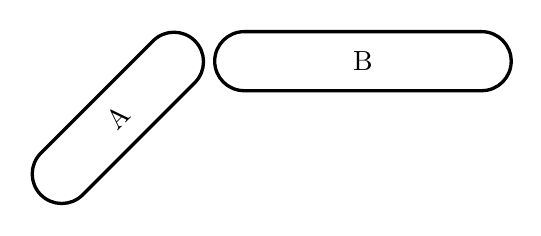
\begin{tikzpicture}

\node[name=A, shape=rounded rectangle, minimum width=3cm, minimum height=0.75cm, rotate=45, anchor=-12.12, very thick, draw] at (-0.05cm,0) {A};
\node[name=B, shape=rounded rectangle, minimum width=4cm, minimum height=0.75cm, rotate=0, anchor=west, very thick, draw] at (0.05cm,0) {B};

\end{tikzpicture}
\end{figure}

The velocity of a point with position $\vec{r}$ relative to the center
of mass of a cell with its main axis along the unit vector $\hat{a}$
is:

\begin{align*}
\vec{v_r} &= \vec{v}_\textrm{linear} + \vec{v}_\textrm{angular} + \vec{v}_\textrm{growth} \\
&= \vec{v} + \vec{\w} \times \vec{r} + \frac{1}{2} \frac{\hat{a} \cdot \vec{r}}{l} v_{growth} \\
&= \vec{v} - \vec{r} \times \vec{\w} + \frac{1}{2} \frac{\hat{a} \cdot \vec{r}}{l} v_{growth} \\
&= \frac{1}{m}\vec{p} - \vec{r} \times \IInv\vec{L} + \frac{1}{2} \frac{\hat{a} \cdot \vec{r}}{l} \frac{g}{G} \\
&= \frac{1}{m}\vec{p} - \rx \IInv\vec{L} + \frac{1}{2} \frac{\hat{a} \cdot \vec{r}}{l} \frac{g}{G} \\
\end{align*}

This expression is linear in $\vec{p}$, $\vec{L}$, and $g$, so the
velocity of the point after an impulse $\deltap$ is:

\begin{align*}
\vec{v_r} &= \vec{v_r}_0 + \deltav \\
&= \vec{v_r}_0 + \frac{1}{m}\deltap - \rx\IInv\deltaL \times \vec{r} + \frac{1}{2} \frac{\hat{x} \cdot \vec{r}}{l} \frac{\deltag}{G} \\
&= \vec{v_r}_0 + \vec{M}_{\hat{a},{\vec{r}}} \deltap
\end{align*}

\dots where:

\[
\vec{M}_{\hat{a},{\vec{r}}}
=
\left[
\begin{array}{ccc}
\frac{1}{m}I & \rx\IInv & \frac{\hat{a}\cdot\vec{r}}{2lG}\hat{a}\\
\end{array}
\right]
\]

\dots and:

\[
\deltap
=
\left[
\begin{array}{c}
\deltap \\
\deltaL \\
\deltag \\
\end{array}
\right]
=
\left[
\begin{array}{c}
\Delta p_x \\
\Delta p_y \\
\Delta p_z \\
\Delta L_x \\
\Delta L_y \\
\Delta L_z \\
\deltag \\
\end{array}
\right]
\]

In the above, $I$ is the identity matrix and $\IInv$ is the inverse
inertia tensor.  No confusion should arise from the use of $\deltap$
to signify both general momentum and specifically linear momentum.

The inertia tensor for a rod of mass $m$, radius $r$, and length $l$
centered at the origin and lying along the $x$ axis is:
\[
\mathbf{I}
=
\frac{1}{12}m
\left[
\begin{array}{ccc}
6r^2 & 0 & 0 \\
0 & 3r^2 + l^2 & 0 \\
0 & 0 & 3r^2 + l^2 \\
\end{array}
\right]
\]

Therefore the inverse inertia tensor for the same cylinder is:
\[
\IInv
=
\frac{12}{m}
\left[
\begin{array}{ccc}
\frac{1}{6r^2} & 0 & 0 \\
0 & \frac{1}{3r^2+l^2} & 0 \\
0 & 0 & \frac{1}{3r^2+l^2} \\
\end{array}
\right]
\]

Suppose $\mathbf{T}_i$ transforms from world coordinates to local
coordinates for cell $i$ --- i.e. it transforms the $x$ axis to the
main axis of that cell.  Then the inverse inertia tensor for cell $i$
in world coordinates is given by:

\[\IInv_i = \mathbf{T}_i \IInv_\textrm{cyl} \mathbf{T}_i^{-1}\]

So we now have:

\[
\vec{M}_{\hat{a},{\vec{r}}}
=
\left[
\begin{array}{ccc}
\frac{1}{m}I &
\rx \mathbf{T}_i \IInv_\textrm{cyl} \mathbf{T}_i^{-1} &
\frac{\hat{a}\cdot\vec{r}}{2lG}\hat{a}\\
\end{array}
\right]
\]


We assume that colliding capsules --- those that overlap and are
moving toward each other (the dot product of the velocity vectors of
the contact points on the two capsules is negative) --- collide
inelastically.  In this case, the relative velocity of the two contact
points along the normal $\hat{n}$ after the impulse provided by the
collision must be zero.  So:

\begin{align*}
\nT\left(\vec{v}_{\vec{r}_a} - \vec{v}_{\vec{r}_b}\right) \cdot &= 0 \\
\nT \vec{M}_{\vec{r}_a} \vec{p}_a - \nT \vec{M}_{\vec{r}_b} \vec{p}_b &= 0 \\
\nT \vec{M}_{\vec{r}_a} \left( \vec{p}_{a_0} + \deltap_a \right) - \nT \vec{M}_{\vec{r}_b} \left( \vec{p}_{b_0} + \deltap_b \right) &= 0 \\
\nT \vec{M}_{\vec{r}_a} \deltap_a - \nT \vec{M}_{\vec{r}_b} \deltap_b &= \nT \vec{M}_{\vec{r}_b} \vec{p}_{b_0} - \nT \vec{M}_{\vec{r}_a} \vec{p}_{a_0} \\
\nT \vec{M}_{\vec{r}_a} \deltap_a - \nT \vec{M}_{\vec{r}_b} \deltap_b &= \nT \vec{v}_{b_0} - \nT \vec{v}_{a_0} \\
\nT \vec{M}_{\vec{r}_a} \deltap_a - \nT \vec{M}_{\vec{r}_b} \deltap_b &= \nT \vec{v}_{\textrm{rel}_{a,b}} \\
\end{align*}

Write:

\begin{align*}
\vec{N}_{\hat{a},{\vec{r}}}
&=
\left[
\begin{array}{ccc}
\nT \frac{1}{m}I &
\nT \rx \mathbf{T}_i \IInv_\textrm{cyl} \mathbf{T}_i^{-1} &
\nT \frac{\hat{a}\cdot\vec{r}}{2lG}\hat{a}\\
\end{array}
\right] \\
&=
\left[
\begin{array}{ccc}
\frac{1}{m} \hat{n} &
\nT \rx \mathbf{T}_i \IInv_\textrm{cyl} \mathbf{T}_i^{-1} &
\frac{1}{2lG}\left(\hat{a}\cdot\vec{r}\right)\left(\hat{a}\cdot\hat{n}\right)\\
\end{array}
\right] \\
\end{align*}

This is a $1\times7$ matrix which when multiplied by the $7\times1$
matrix $\deltap$ gives a change in velocity along the normal $\hat{n}$.



In block matrix form, we can write:

\[
\left[
\begin{array}{cc}
\nT\vec{M}_{\vec{r}_a} & -\nT\vec{M}_{\vec{r}_b} \\
\end{array}
\right]
\left[
\begin{array}{c}
\deltap_a \\
\deltap_b \\
\end{array}
\right]
=
\nT\vec{v}_{\textrm{rel}_{a,b}}
\]

More generally, we will have a system of equations with one such
equation for each pair of colliding cells.  We build a larger block
matrix with a row for each constraint and a column for each cell in
the system.  If the $i$th constraint involves cells $a$ and $b$ (in
that order), then:

\[\vec{M}_{ij} = \left\{
\begin{array}{ll}
\nT\vec{M}_{\vec{r}_a} & \textrm{if } j=a \\
-\nT\vec{M}_{\vec{r}_b} & \textrm{if } j=b \\
0 & \textrm{otherwise} \\
\end{array}
\right\}\]


A sytem with four cells and four collisions might have the equation:

\[
\left[
\begin{array}{cccc}
\vec{M}_{\vec{r}_{1a}} & -\vec{M}_{\vec{r}_{1b}} & 0 & 0 \\
0 & \vec{M}_{\vec{r}_{2b}} & -\vec{M}_{\vec{r}_{2c}} & 0 \\
\vec{M}_{\vec{r}_{3a}} & 0 & 0 & -\vec{M}_{\vec{r}_{3d}} \\
0 & 0 & \vec{M}_{\vec{r}_{4c}} & -\vec{M}_{\vec{r}_{4d}} \\
\end{array}
\right]
\left[
\begin{array}{c}
\deltap_a \\
\deltap_b \\
\deltap_c \\
\deltap_d \\
\end{array}
\right]
=
\left[
\begin{array}{c}
\vec{v}_{\textrm{rel}_{a,b}} \\
\vec{v}_{\textrm{rel}_{b,c}} \\
\vec{v}_{\textrm{rel}_{a,d}} \\
\vec{v}_{\textrm{rel}_{c,d}} \\
\end{array}
\right]
\]


We can transform this into a square matrix by multiplying by $\vec{M}^\textrm{T}$.

\[
\vec{M}^\textrm{T} \vec{M} \deltap = \vec{M}^\textrm{T} \vec{v}_{\textrm{rel}}
\]

Consider $\vec{A} = \vec{M}^\textrm{T} \vec{M}$.  We have:

\[
\vec{A}_{ij} = \sum_{k} \vec{M}^\textrm{T}_{ik} \vec{M}_{kj}
\]

\dots where $k \in \textrm{constraints}$.

If $i \neq j$ and there is no constraint between cells $i$ and $j$
then ${\vec{M}^\textrm{T}}_{ik} \vec{M}_{kj}$ will be zero.  If there
is a constraint between $i$ and $j$, then:

\[
\vec{A}_{ij} = -\vec{M}^\textrm{T}_{\vec{r}_{ik}} \vec{M}_{\vec{r}_{jk}}
\]

\dots where $\vec{r}_{ik}$ is the vector from the center of cell $i$
to the point on the surface of that cell associated with contact $k$.

If $i=j$, then:

\[
\vec{A}_{ii} = \sum_k{\vec{M}^\textrm{T}_{\vec{r}_{ik}}\vec{M}_{\vec{r}_{ik}}}
\]

\dots where $k$ ranges over all constraints involving cell $i$.

In general:

\[
\vec{M}_\vec{s}^\textrm{T} \vec{M}_\vec{r}
=
\begin{bmatrix*}
\frac{1}{M_1M_2} & 0 & 0 & 0 & \frac{\vec{s}_z}{I_2} & -\frac{\vec{s}_y}{I_2} & \frac{{\vec{a}_\vec{s}}_x}{2l_2G_2} \\[6pt]
0 & \frac{1}{M_1M_2} & 0 & -\frac{\vec{s}_z}{I_2} & 0 & \frac{\vec{s}_x}{I_2} & \frac{{\vec{a}_\vec{s}}_y}{2l_2G_2} \\[6pt]
0 & 0 & \frac{1}{M_1M_2} & \frac{\vec{s}_y}{I_2} & -\frac{\vec{s}_x}{I_2} & 0 & \frac{{\vec{a}_\vec{s}}_z}{2l_2G_2} \\[6pt]
0 & -\frac{\vec{r}_z}{I_1} & \frac{\vec{r}_y}{I_1} & \frac{\vec{r}_y\vec{s}_y + \vec{r}_z\vec{s}_z}{I_1I_2} & -\frac{\vec{r}_y\vec{s}_x}{I_1I_2} & -\frac{\vec{r}_z\vec{s}_x}{I_1I_2} & \frac{\vec{r}_y{\vec{a}_\vec{s}}_z}{2I_1l_2G_2} \\[6pt]
\frac{\vec{r}_z}{I_1} & 0 & -\frac{\vec{r}_x}{I_1} & -\frac{\vec{r}_x\vec{s}_y}{I_1I_2} & \frac{\vec{r}_x\vec{s}_x + \vec{r}_z\vec{s}_z}{I_1I_2} & -\frac{\vec{r}_z\vec{s}_y}{I_1I_2} & \frac{\vec{r}_z{\vec{a}_\vec{s}}_x}{2I_1l_2G_2} \\[6pt]
-\frac{\vec{r}_y}{I_1} & \frac{\vec{r}_x}{I_1} & 0 & -\frac{\vec{r}_x\vec{s}_z}{I_1I_2} & -\frac{\vec{r}_y\vec{s}_z}{I_1I_2} & \frac{\vec{r}_y\vec{s}_y + \vec{r}_z\vec{s}_z}{I_1I_2} & \frac{\vec{r}_x{\vec{a}_\vec{s}}_y}{2I_1l_2G_2} \\[6pt]
\frac{{\vec{a}_\vec{r}}_x}{2l_1G_1} & \frac{{\vec{a}_\vec{r}}_y}{2l_1G_1} & \frac{{\vec{a}_\vec{r}}_z}{2l_1G_1} &
\frac{\vec{s}_y{\vec{a}_\vec{r}}_z - \vec{s}_z{\vec{a}_\vec{r}}_y}{2I_2l_1G_1} &
\frac{\vec{s}_z{\vec{a}_\vec{r}}_x - \vec{s}_x{\vec{a}_\vec{r}}_z}{2I_2l_1G_1} &
\frac{\vec{s}_x{\vec{a}_\vec{r}}_y - \vec{s}_y{\vec{a}_\vec{r}}_x}{2I_2l_1G_1} &
\frac{\vec{a}_\vec{r} \cdot \vec{a}_\vec{s}}{4l_1l_2G_1G_2} \\
\end{bmatrix*}
\]

\dots and:

\[
\vec{M}_\vec{r}^\textrm{T} \vec{M}_\vec{r}
=
\begin{bmatrix*}
\frac{1}{M_1^2} & 0 & 0 & 0 & \frac{\vec{r}_z}{I_1} & -\frac{\vec{r}_y}{I_1} & \frac{{\vec{a}_\vec{r}}_x}{2l_1G_1} \\
0 & \frac{1}{M_1^2} & 0 & -\frac{\vec{r}_z}{I_1} & 0 & \frac{\vec{r}_x}{I_1} & \frac{{\vec{a}_\vec{r}}_y}{2l_1G_1} \\
0 & 0 & \frac{1}{M_1^2} & \frac{\vec{r}_y}{I_1} & -\frac{\vec{r}_x}{I_1} & 0 & \frac{{\vec{a}_\vec{r}}_z}{2l_1G_1} \\
0 & -\frac{\vec{r}_z}{I_1} & \frac{\vec{r}_y}{I_1} & \frac{\vec{r}_y^2 + \vec{r}_z^2}{I_1^2} & -\frac{\vec{r}_y\vec{r}_x}{I_1^2} & -\frac{\vec{r}_z\vec{r}_x}{I_1^2} & \frac{\vec{r}_y{\vec{a}_\vec{r}}_z}{2I_1l_1G_1} \\
\frac{\vec{r}_z}{I_1} & 0 & -\frac{\vec{r}_x}{I_1} & -\frac{\vec{r}_x\vec{r}_y}{I_1^2} & \frac{\vec{r}_x^2 + \vec{r}_z^2}{I_1^2} & -\frac{\vec{r}_z\vec{r}_y}{I_1^2} & \frac{\vec{r}_z{\vec{a}_\vec{s}}_x}{2I_1l_1G_1} \\
-\frac{\vec{r}_y}{I_1} & \frac{\vec{r}_x}{I_1} & 0 & -\frac{\vec{r}_x\vec{r}_z}{I_1^2} & -\frac{\vec{r}_y\vec{r}_z}{I_1^2} & \frac{\vec{r}_y^2 + \vec{r}_z^2}{I_1^2} & \frac{\vec{r}_x{\vec{a}_\vec{r}}_y}{2I_1l_1G_1} \\
\frac{{\vec{a}_\vec{r}}_x}{2l_1G_1} & \frac{{\vec{a}_\vec{r}}_y}{2l_1G_1} & \frac{{\vec{a}_\vec{r}}_z}{2l_1G_1} &
\frac{\vec{r}_y{\vec{a}_\vec{r}}_z - \vec{r}_z{\vec{a}_\vec{r}}_y}{2I_1l_1G_1} &
\frac{\vec{r}_z{\vec{a}_\vec{r}}_x - \vec{r}_x{\vec{a}_\vec{r}}_z}{2I_1l_1G_1} &
\frac{\vec{r}_x{\vec{a}_\vec{r}}_y - \vec{r}_y{\vec{a}_\vec{r}}_x}{2I_1l_1G_1} &
\frac{\vec{a}_\vec{r} \cdot \vec{a}_\vec{r}}{4l_1^2G_1^2} \\
\end{bmatrix*}
\]

\dots where:

\begin{align*}
\vec{a}_\vec{r} &= \left(\hat{x}_1 \cdot \vec{r}\right) \vec{r} \\
\vec{a}_\vec{s} &= \left(\hat{x}_2 \cdot \vec{s}\right) \vec{s} \\
\end{align*}

So we are left with the equation:

\[
\vec{A}\deltap = \deltav
\]

\dots where:

\[
\vec{A}_{ij} = \left\{
  \begin{array}{ll}
    \vec{M}^\textrm{T}_i\vec{M}_i & \textrm{if } i = j \\
    -\vec{M}^\textrm{T}_i\vec{M}_j & \textrm{if cell } i \textrm{ and cell } j \textrm{ are colliding} \\
  \end{array}\right\}
\]




\end{document}
